\section{Grundschwingungen}

Die Grundschwingungen stellen Schwingungszustände dar, in denen das System mit einer Frequenz schwingt. Dies lässt sich darstellen, durch eine Funktion der Art:\\
\begin{align}
f(x)= a \cdot e^{-bt} \sin(\omega t+d)+c
\end{align} 
Diese wird nun an die jeweiligen Messungen, mit Hilfe von "Gnuplot" angepasst. 
Unsicherheiten entstehen durch das Auflösevermögen (\SI{1}{cm}) des Entfernungsmessers "Motion Sensor" von "Pasco" sowie der Zeitmessung. Die Quarzuhr des Computers hat eine Ungenauigkeit der Größenordnung \footnote{entnommen aus: https://de.wikipedia.org/wiki/Quarzuhr} $10^{-5}$ und ist somit gegenüber den statistischen Abweichungen der Größenordnung $10^{-4}$ zu vernachlässigen. Aus dem Auflösevermögen des Entfernungsmessers ergibt sich nach Gleichung \ref{eq:SR} eine Unsicherheit der Amplitude von $\Delta a= \SI{0.003}{m}$
\subsection{Gleichsinnige Bewegung}
\subsubsection*{Kupferfeder}


\begin{figure}[h!]
	\centering
	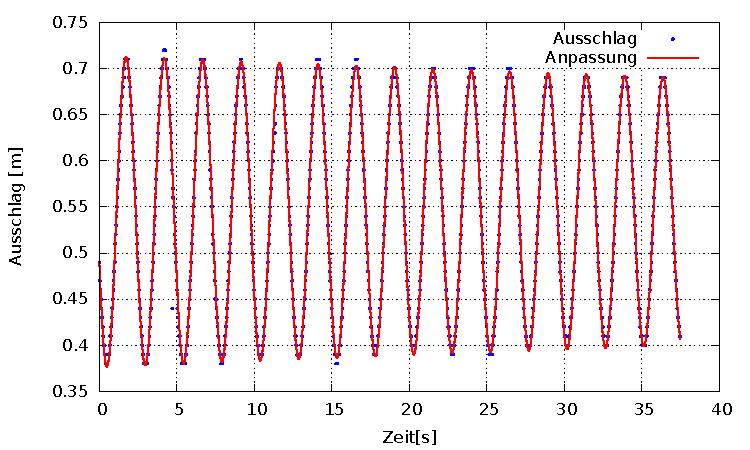
\includegraphics[width=0.7\linewidth]{Auswertung/kupfer/gleich/kupferglA}
	\caption{Die Abbildung zeigt die Auslenkung des rechten Pendels, bei Koppelung durch eine Kupferfeder, in der Horizontalen. Beide Pendel wurden zu Beginn so ausgelenkt, dass sie gleichsinnig, also in Phase, Schwingen. }
	\label{fig:kupfergl}
\end{figure}

\begin{align*}
	a               &= \SI{-0.168666       \pm 0.000427 }{m}    \\
	\rho               &= \SI{0.0040146      \pm 0.0001221}{\per \second}    \\
	\omega               &= \SI{2.53782          \pm 0.0001224}{\per \second}   \\
	\varphi              & = 0.338584        \pm  0.002559     \\
	c              & = 0.545177     \pm  0.0001464    \\
\end{align*}


Es ist zu erkennen, dass die Messpunkte nahezu vollständig in zu der Anpassung passen. Bis auf einen Punkt sind alle Ausreißer um weniger als eine Anzeigeschritt von der Kurve entfernt. Bei dem Punkt um $t=\SI{5}{s}$ ist von einem Datenverarbeitungsfehler seitens des Programms auszugehen, diese nahmen mit steigender Frequenz zu, kamen jedoch auch schon bei \SI{50}{Hz} vor. Wir erhalten nach Gleichung\ref{eq:T} eine Periodendauer von $T_{gl}= \SI{2.47582 \pm 0.00012}{s}$



\subsubsection*{Edelstahlfeder}



\begin{figure}[h!]
	\centering
	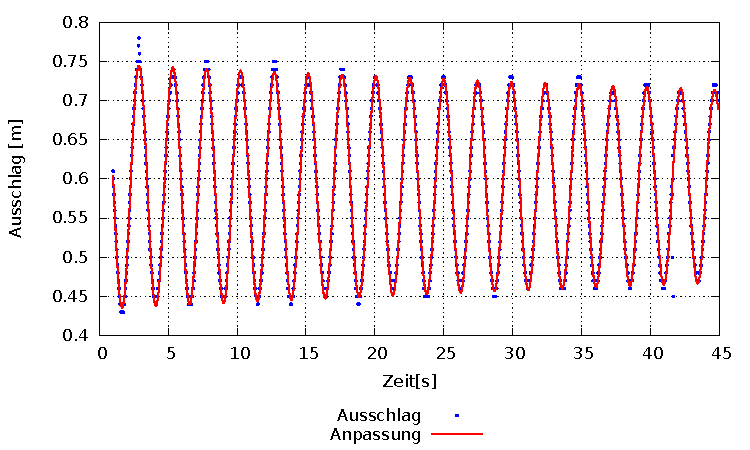
\includegraphics[width=0.7\linewidth]{Auswertung/stahl/gleich/stahlglA}
	\caption{Die Abbildung zeigt die Auslenkung des rechten Pendels, bei Koppelung durch eine Edelstahlfeder, in der Horizontalen. Beide Pendel wurden zu Beginn so ausgelenkt, dass sie gleichsinnig, also in Phase, Schwingen.}
	\label{fig:stahlgl}
\end{figure}

\begin{align*}
a               &= \SI{ -0.12632        \pm 0.0021  }{m}     \\
\rho               &=\SI{ -0.00177149     \pm 0.0006273}{\per s}    \\
\omega               &= \SI{2.55753         \pm 0.0006423 }{\per s}    \\
\varphi               &= 3.59422         \pm 0.01692     \\
c               &=\SI{ 0.586199        \pm 0.0007644}{m}     \\
\end{align*}



\subsection{Gegensinnige Bewegung}




\subsubsection*{Kupferfeder}


\begin{figure}[h!]
	\centering
	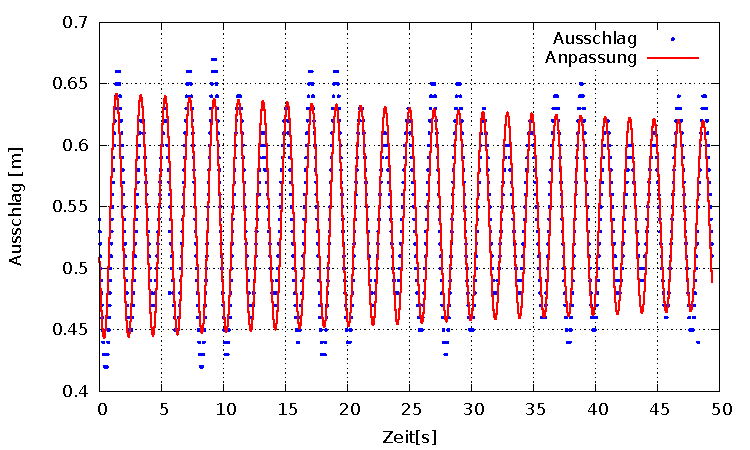
\includegraphics[width=0.7\linewidth]{Auswertung/kupfer/gegen/1/kupfergegA}
	\caption{Die Abbildung zeigt die Auslenkung des rechten Pendels, bei Koppelung durch eine Kupferfeder, in der Horizontalen. Beide Pendel wurden zu Beginn so ausgelenkt, dass sie gegensinnig Schwingen.}
	\label{fig:kupfergega}
\end{figure}


\begin{align*}
a               &=\SI{  -0.0997614      \pm 0.001289 }{m}    \\
\rho              &=\SI{  0.00528663      \pm 0.0004877 }{\per s}    \\
\omega              &=\SI{  3.1857          \pm 0.0004867 }{\per s}   \\
\varphi               &=  0.355226        \pm 0.013       \\
c              &=\SI{  0.542896        \pm 0.000429  }{m}    \\
\end{align*}



\subsubsection*{Edelstahlfeder}



\begin{figure}[h!]
	\centering
	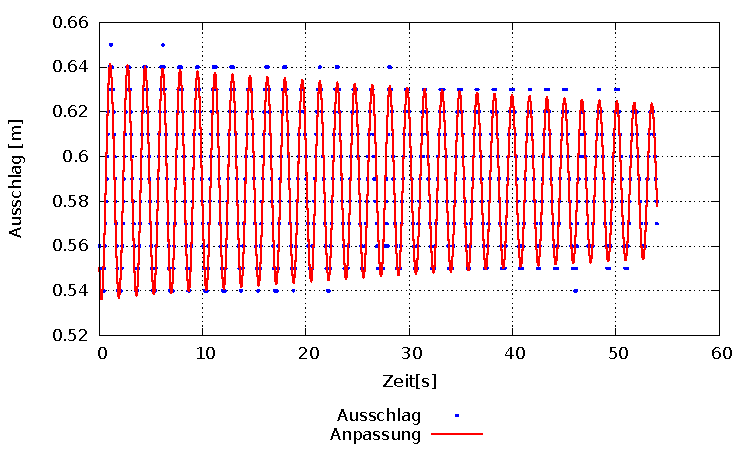
\includegraphics[width=0.7\linewidth]{Auswertung/stahl/gegen/stahlgegA}
	\caption{Die Abbildung zeigt die Auslenkung des rechten Pendels, bei Koppelung durch eine Edelstahlfeder, in der Horizontalen. Beide Pendel wurden zu Beginn so ausgelenkt, dass sie gegensinnig Schwingen.}
	\label{fig:stahlgega}
\end{figure}

\begin{align*}
a               =\SI{ -0.0527356      \pm 0.00039  }{m}    \\
\rho               =\SI{ 0.0079019       \pm 0.0002681}{\per s}    \\
\omega               = \SI{3.71409         \pm 0.0002692}{\per s}    \\
\varphi               = 0.829914        \pm 0.007483    \\
c              = \SI{0.58904         \pm 0.0001252  }{m}  \\
\end{align*}






